\documentclass{exam}
\usepackage[utf8]{inputenc}
\usepackage{lmodern}
\usepackage{microtype}

% \usepackage[parfill]{parskip}
\usepackage[dvipsnames]{xcolor}
\usepackage{amsmath}
\usepackage{amsfonts}
\usepackage{amsthm}
\usepackage{siunitx}
\DeclareSIUnit\year{yr}
\DeclareSIUnit\foot{ft}
\DeclareSIUnit\litre{\liter}

\usepackage{skull}

\usepackage{pgfplots}
\usepgfplotslibrary{polar}
\pgfplotsset{compat=1.11}
\usepgfplotslibrary{statistics}
\usepackage{graphicx}
\usepackage{sidecap}
\sidecaptionvpos{figure}{c}
\usepackage{float}
\usepackage{gensymb}
\usepackage{tkz-euclide}
\usetkzobj{all}
\usepackage{commath}
\usepackage{hyperref}
\usepackage{enumitem}
\usepackage{wasysym}
\usepackage{multicol}
\usepackage{mathtools}
\usepackage{tcolorbox}
\usepackage{tabularx}
\usepackage[version=4]{mhchem}
\usepackage{changepage}
\usepackage{listings}
\lstset{basicstyle=\ttfamily\linespread{0.8}\small}

\renewcommand*{\thefootnote}{\fnsymbol{footnote}}

\newtheorem*{thm}{Theorem}
\newtheorem*{iden}{Identity}
\newtheorem*{lemma}{Lemma}
\newtheorem{obs}{Observation}
\theoremstyle{definition}
\newtheorem*{defn}{Definition}
\newtheorem*{ex}{Example}
\newtheorem{con}{Construction}
\newtheorem*{alg}{Algorithm}

\newtheoremstyle{break}
  {\topsep}{\topsep}%
  {\itshape}{}%
  {\bfseries}{}%
  {\newline}{}%
\theoremstyle{break}
\newtheorem*{bthm}{Theorem}

% russian integral
\usepackage{scalerel}
\DeclareMathOperator*{\rint}{\scalerel*{\rotatebox{17}{$\!\int\!$}}{\int}}

% \DeclareMathOperator*{\rint}{\int}

\pgfplotsset{vasymptote/.style={
    before end axis/.append code={
        \draw[densely dashed] ({rel axis cs:0,0} -| {axis cs:#1,0})
        -- ({rel axis cs:0,1} -| {axis cs:#1,0});
    }
}}

% \pointsinrightmargin
\boxedpoints
\pointname{}

\newcommand{\questioA}{\question[\texttt{\textbf{\color{Cerulean} A}}]}
\newcommand{\questioM}{\question[\texttt{\textbf{\color{PineGreen} M}}]}
\newcommand{\questioE}{\question[\texttt{\textbf{\color{WildStrawberry} E}}]}
\newcommand{\questioS}{\question[\texttt{\textbf{\color{Goldenrod} S}}]}
\newcommand{\questioO}{\question[\texttt{\textbf{\color{BurntOrange} O}}]}

\newcommand{\parA}{\part[\texttt{\textbf{\color{Cerulean} A}}]}
\newcommand{\parM}{\part[\texttt{\textbf{\color{PineGreen} M}}]}
\newcommand{\parE}{\part[\texttt{\textbf{\color{WildStrawberry} E}}]}
\newcommand{\parS}{\part[\texttt{\textbf{\color{Goldenrod} S}}]}
\newcommand{\parO}{\part[\texttt{\textbf{\color{BurntOrange} O}}]}

\newcommand{\subparA}{\subpart[\texttt{\textbf{\color{Cerulean} A}}]}
\newcommand{\subparM}{\subpart[\texttt{\textbf{\color{PineGreen} M}}]}
\newcommand{\subparE}{\subpart[\texttt{\textbf{\color{WildStrawberry} E}}]}
\newcommand{\subparS}{\subpart[\texttt{\textbf{\color{Goldenrod} S}}]}
\newcommand{\subparO}{\subpart[\texttt{\textbf{\color{BurntOrange} O}}]}

\newcommand{\mainHeader}[2]{\section*{NCEA Level 2 Mathematics\\#1. #2}}
\newcommand{\mainHeaderHw}[2]{\section*{NCEA Level 2 Mathematics (Homework)\\#1. #2}}
\newcommand{\seealso}[1]{\begin{center}\emph{See also #1.}\end{center}}
\newcommand{\drills}[1]{\begin{center}\emph{Drill problems: #1.}\end{center}}
\newcommand{\basedon}[1]{\begin{center}\emph{Notes largely based on #1.}\end{center}}


\begin{document}

\mainHeaderDiffHw{1}{The Derivative}
\subsection*{Reading}
\textit{From \textit{Calculus Made Easy}, by Silvanus P. Thompson and revised by Martin Gardner}

Considering how many fools can calculate, it is surprising that it should be thought a difficult or
a tedious task for any other fool to learn how to master the same tricks.

Some calculus-tricks are quite easy. Some are enormously difficult. The fools who write the text-books
of advanced mathematics --- and they are mostly clever fools --- seldom take the time to show you how
easy the easy calculations are. On the contrary, they seem to desire to impress you with their tremendous
cleverness by going about it in the most difficult way.

Being myself a remarkably stupid fellow, I have had to unteach myself the difficulties, and now beg
to present to my fellow fool the parts that are not hard. Master these thoroughly, and the rest will
follow. What one fool can do, another can.

The preliminary terror, which chokes off most high school students from even attempting to learn
how to calculate, can be abolished once and for all by simply stating what is the meaning --- in
common-sense terms --- of the two principal symbols that are used in calculating.

These dreadful symbols are:

(1) $ \dif{} $, which merely means "a little bit of".

Thus $ \dif{x} $ meas a little bit of $ x $;
or $ \dif{u} $ means a little bit of $ u $. Ordinary mathematicians think it more polite to say
"an element of", instead of "a little bit of". Just as you please. But you will find that these
little bits (or elements) may be considered to be infinitesimally small.

(2) $ \rint $, which is merely a long $ S $, and may be called (if you like) "the sum of".

Thus $ \rint \dif{x} $ means the sum of all the little bits of $ x $; or $ \rint \dif{t} $ means
the sum of all the little bits of $ t $. Ordinary mathematicians call this symbol "the integral of".
Now any fool can see that if $ x $ is considered to be made up of a lot of little bits, each of
which is called $ \dif{x} $, if you add them all up together you get the sum of all the $ \dif{x}$'s (which
is simply the same thing as the whole of $ x $). The word "integral" simply means "the whole". If you think
of the duration of time for one hour, you may  (if you like) think of it cut up into 3600 little bits
called seconds. The whole of the 3600 little bits added up together make one hour.

When you see an expression that begins with this terrifying symbol, you will henceforth know that it is put
there merely to give you instructions that you are now to perform the operation (if you can) of totalling up
all the little bits that are indicated by the symbols that follow.

That's all.

\clearpage
\subsection*{Questions}
\begin{questions}
  \question Given that the following graph is the derivative of a function passing through $ (0,0) $, draw the original function.
      \begin{center}
        \fbox{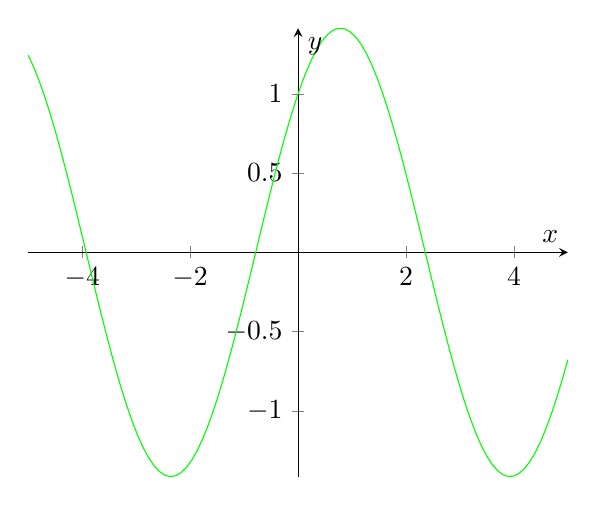
\begin{tikzpicture}
          \begin{axis}[
            axis lines = center,
            xlabel = $ x $,
            ylabel = $ y $
          ]
            \addplot[domain = -5:5, color = green, samples=100] {sin(deg(x)) + cos(deg(x))};
          \end{axis}
        \end{tikzpicture}}
      \end{center}
  \question
    \begin{parts}
      \part At a maxima or minima, what value $ m $ does the derivative of a function take? Explain this geometrically.
      \part Show, by example (i.e. draw a graph), that there exist functions such that they have a derivative
            equal to $ m $ at a point but not a minimum or maximum at that point.
    \end{parts}
\end{questions}
\end{document}
